\documentclass[utf8, 12pt]{beamer}
\usepackage[utf8]{inputenc}
\usepackage[russian]{babel}

\usepackage{eulervm}

%выбор темы
\usetheme{Madrid}
\useoutertheme{shadow}
\beamertemplatenavigationsymbolsempty
\setbeamertemplate{footline}[frame number]

\usepackage{fontspec}
\defaultfontfeatures{Scale=MatchLowercase}
\setmainfont[Mapping=tex-text]{Liberation Serif}
\setsansfont[Mapping=tex-text]{Liberation Sans}
\setmonofont{Droid Sans Mono}

% переопределяем окружение verbatim
\makeatletter 
\renewcommand*\verbatim@font{% 
\normalfont\ttfamily\small 
\hyphenchar\font\m@ne 
\let\do\do@noligs \verbatim@nolig@list 
} 
\makeatother 

\title{Трассировка лучей в реальном времени \\ на~x64~архитектуре}
\author{}\date{}

\begin{document}
\begin{frame}
\begin{center}
{\tiny
Министерство образования и науки Российской Федерации\\ 
Государственное образовательное учреждение \\ 
высшего профессионального образования \\ 
<<Нижегородский государственный университет им. Н.И. Лобачевского>>\\
\bf{Факультет вычислительной математики и кибернетики \\
Кафедра математического обеспечения ЭВМ} \\
}
\end{center}
\titlepage
\vspace*{-1.75cm}
{\footnotesize
\begin{flushright}
\begin{tabular}{l}
\bf{Исполнитель}: \\ 
магистрант группы 86М1 \\
Морозов Андрей Сергеевич \\
\bf{Научный руководитель}: \\
д. т. н., профессор кафедры МО ЭВМ \\
Турлапов Вадим Евгеньевич
\end{tabular}
\end{flushright}
}
\vspace*{1.2cm}
\begin{center}
\footnotesize Нижний Новгород, 2011г.
\end{center}
\end{frame}

\begin{frame}
\frametitle{Постановка задачи}
Разработать, реализовать и исследовать высокопроизводительный алгоритм трассировки лучей на центральном процессоре:
\begin{itemize}
\item алгоритмическая оптимизация (ускоряющие структуры)
\item параллелизм на уровне данных
\item параллелизм на уровне команд
\end{itemize}
\end{frame}

\begin{frame}
\frametitle{Трассировка лучей}
\begin{itemize}
\item Алгоритм обратной трассировки лучей
\begin{itemize}
\item Модель Фонга
$$
 \vec{I}_{local} =  K_{amb} \cdot \vec{I}_{amb} +  K_{diff} \cdot \vec{I}_{diff} \cdot \left( \vec{L},\vec{N} \right) + K_{spec} \cdot \vec{I}_{spec} \cdot \left( \vec{R},\vec{V} \right)^n
$$
$$
 \vec{I}_{total} = \vec{I}_{local} + K_{reflection} \cdot \vec{I}_{reflection} + K_{refraction} \cdot \vec{I}_{refraction}
$$
\item Теневые лучи
\item Расчет отражений
$$
\vec{R} = \vec{I} - 2 \cdot \vec{N} (\vec{N} , \vec{I})
$$
\end{itemize}
\end{itemize}
\end{frame}


\begin{frame}
\frametitle{Оптимизация}
\begin{itemize}
\item Алгоритмическая оптимизация
\begin{itemize}
\item BVH 
\end{itemize}

\item Параллелизм на уровне данных
\begin{itemize}
\item OpenMP, TBB
\end{itemize}

\item Параллелизм на уровне команд
\begin{itemize}
\item \mbox{\hbox to 2cm {SSE 957}}
\item \mbox{\hbox to 2cm {SS2 403}}
\item \mbox{\hbox to 2cm {SSE3 26}}
\item \mbox{\hbox to 2cm {SSE4.1 82}}
\end{itemize}
\end{itemize}
\end{frame}

\begin{frame}
\frametitle{Результаты}
\begin{itemize}
\item Supersampling
\end{itemize}
\vspace{-2mm}
\begin{figure}[H]
\centering

\includegraphics[scale=3]{imgs/aa_no.png}  \ 

\includegraphics[scale=3]{imgs/aa_my.png}

\includegraphics[scale=3]{imgs/aa_std.png}
\end{figure}
\begin{figure}[H]
\centering
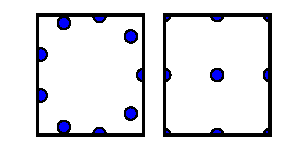
\includegraphics[scale=0.5]{imgs/aa_pattern.pdf}
\end{figure}
\end{frame}

\begin{frame}
\frametitle{Тестовый стенд}
\begin{itemize}
\item CPU
\begin{itemize}
\item Intel Core i7 980X @ 3.33GHz
\item MMX, SSE(1, 2, 3, 3S, 4.1, 4.2), EM64T, VT-x, AES
\item Cores/Threads : 6 / 12
\item L1/L2/L3 : 6 x 32 KBytes / 6 x 256 KBytes / 12 MBytes
\end{itemize}
\item RAM
\begin{itemize}
\item 1066 MHz
\item 6 x 2 GB
\end{itemize}
\item OC
\begin{itemize}
\item Calculate Linux 11.3 x64 
\item Kernel : 2.6.38.6
\end{itemize}
\end{itemize}
\end{frame}

\begin{frame}
\frametitle{Сцена}
\begin{itemize}
\item сфера
\item меш -- набор треугольников 
\item итого : 10817 объектов
\end{itemize}

\def\lllen{1.20cm}
\begin{center}
{\noindent \scriptsize
\begin{tabular}{|r|p{\lllen}|p{\lllen}|p{\lllen}|p{\lllen}|p{\lllen}|}
\hline
Название режима & Ширина изображения &  Высота изображения  & Кол-во субпикселей & Глубина трассировки & Кол-во источников света \\  \hline
low       & 512  & 512  & 1 & 1 & 1 \\ \hline
middle    & 800  & 600  & 2 & 2 & 1 \\ \hline
hard      & 1024 & 768  & 3 & 4 & 2 \\ \hline
very hard & 1920 & 1080 & 3 & 8 & 2 \\ \hline
\end{tabular}
}
\end{center}
\end{frame}

\begin{frame}
\frametitle{Результаты}
\begin{figure}[H]
\centering
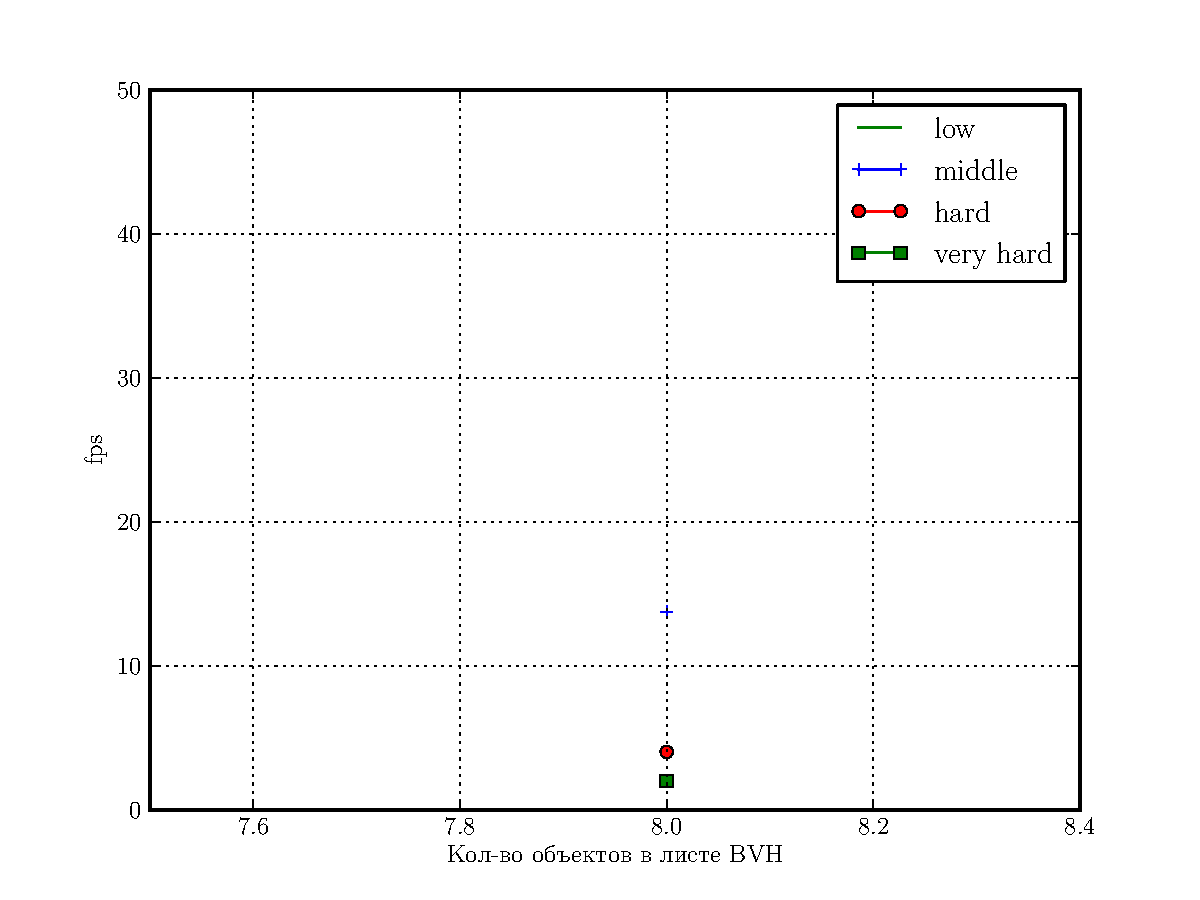
\includegraphics[width=0.9\textwidth]{perf/performance_bvh.pdf}
\end{figure}

\end{frame}

\begin{frame}
\frametitle{Результаты}
\begin{figure}[H]
\centering
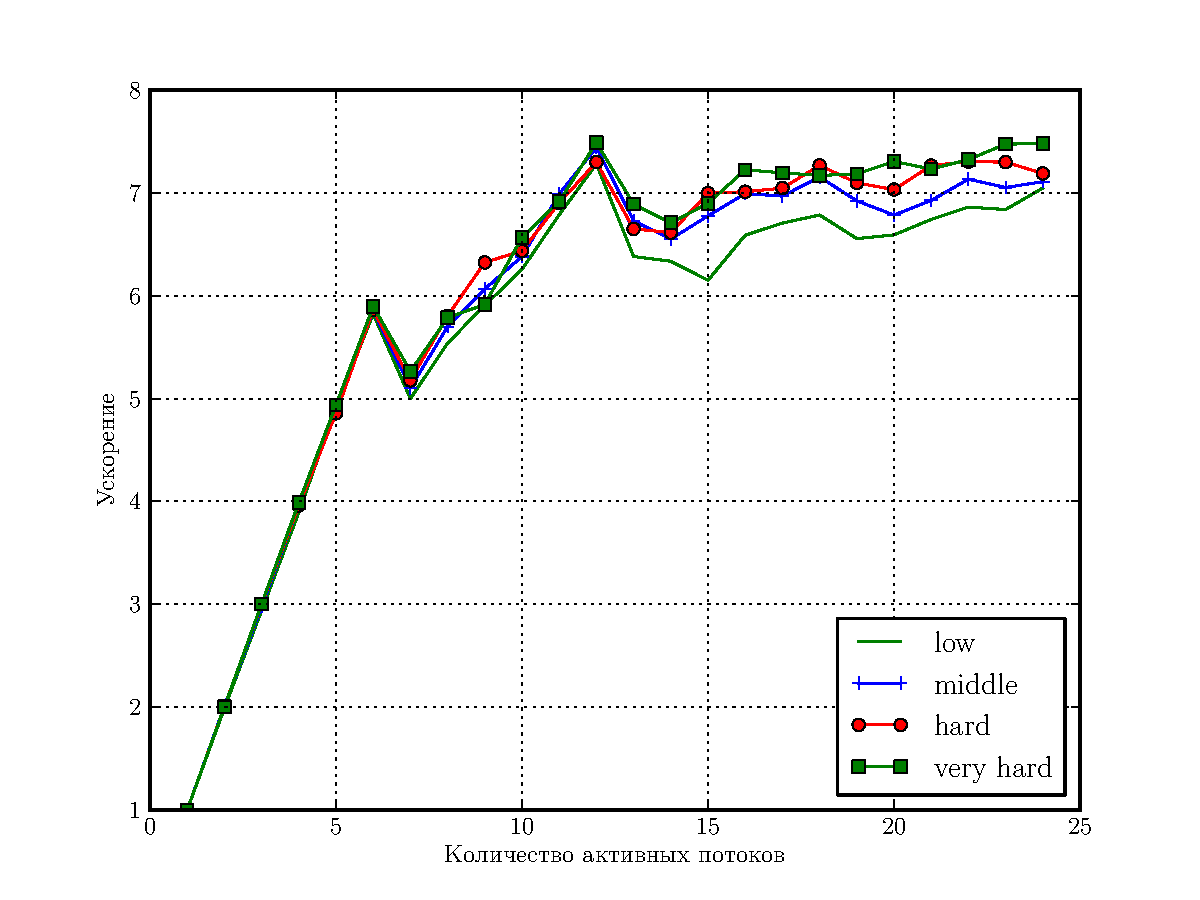
\includegraphics[width=0.9\textwidth]{perf/table_perf_eff.pdf}
\end{figure}
\end{frame}

\begin{frame}
\frametitle{Итоговое изображение}
%\vspace{-5mm}
\begin{figure}[H]
\centering
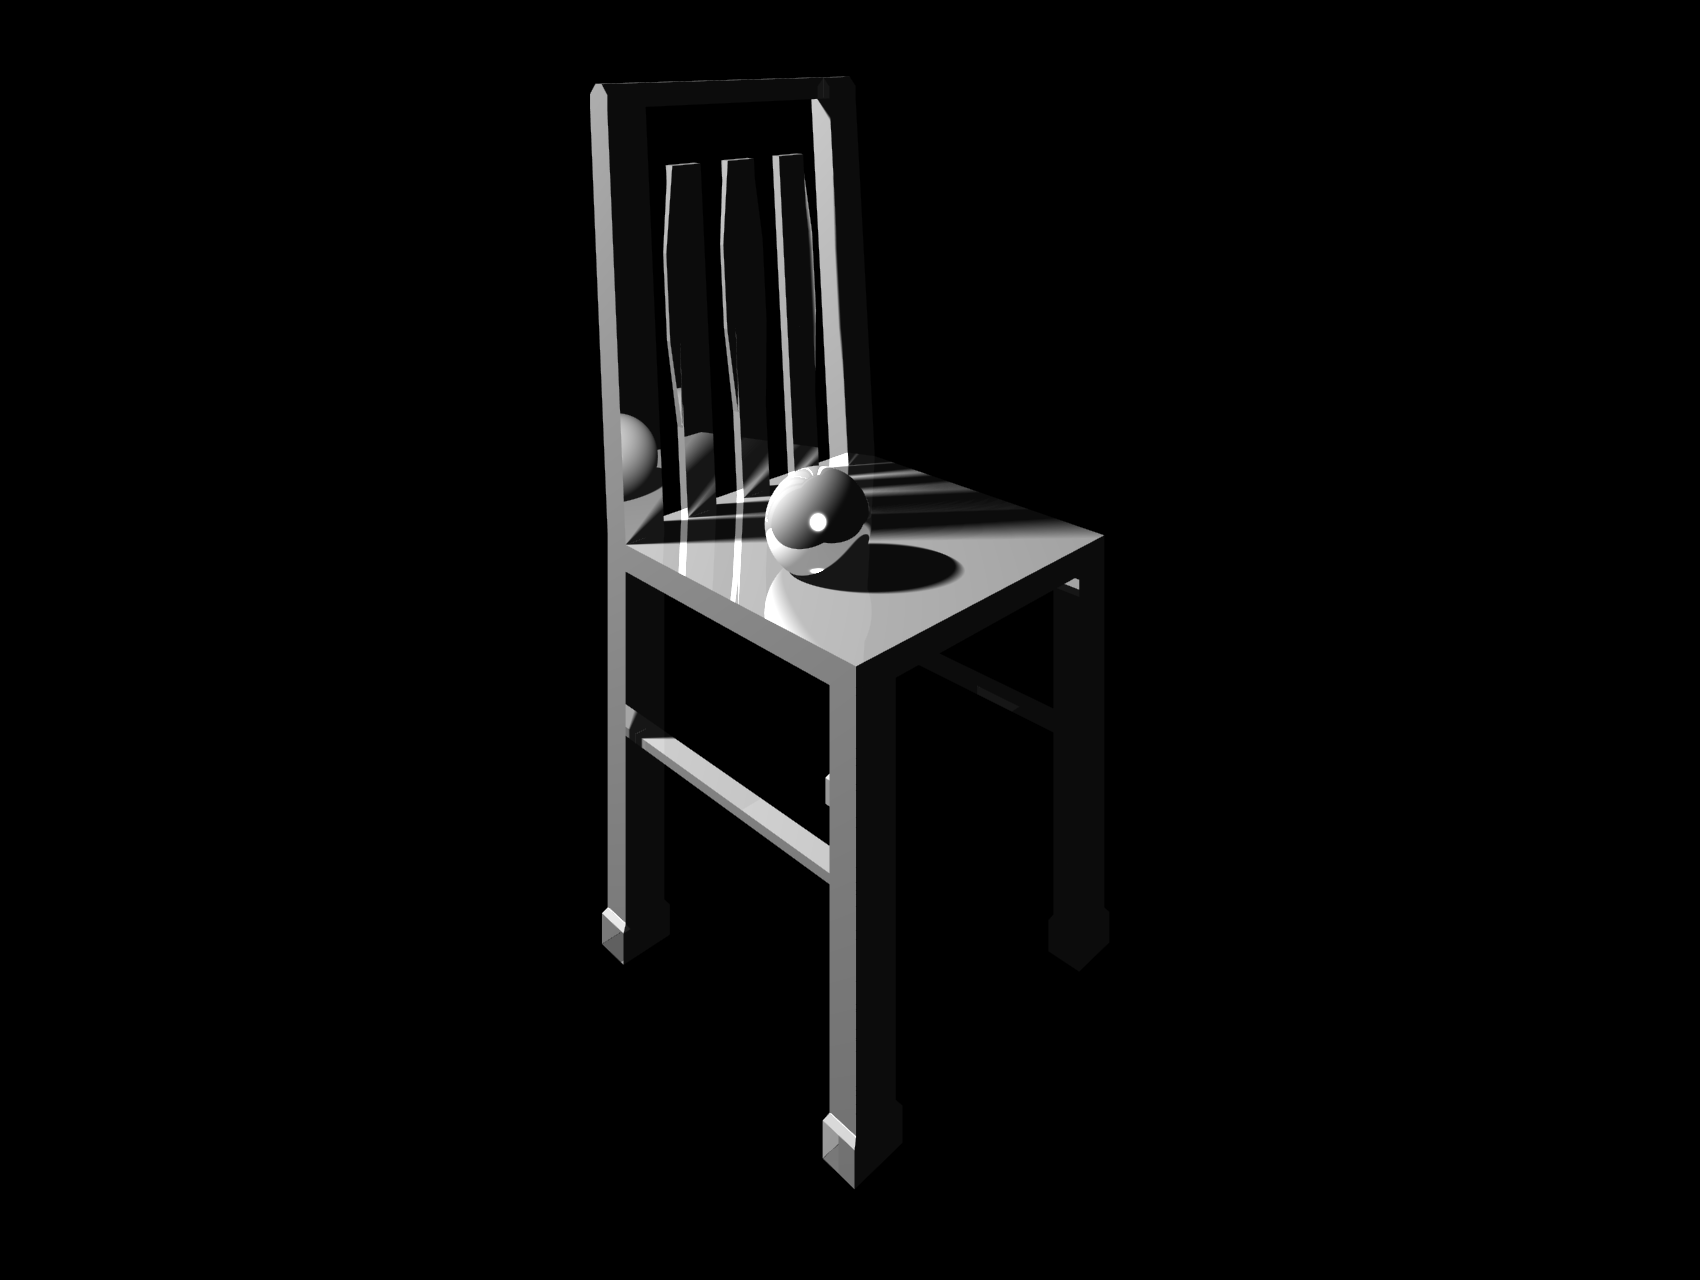
\includegraphics[scale=0.16]{imgs/stulb.png}
\end{figure}

\end{frame}

\begin{frame}
\frametitle{Заключение}
\begin{itemize}
\item Удалось реализовать высокопроизводительный алгоритм трассировки лучей
\begin{itemize}
\item Разрешение : 640х480
\item Объектов в сцене : 10817
\item Глубина трассировки : 16 
\item Итоговая производительность : 36 fps
\end{itemize}
\item Основной вклад в ускорение алгоритма:
\begin{itemize}
\item BVH ( 12 -- 13 раз )
\item OpenMP ( 5 -- 7.6 раз ) ( Hyper-Threading $\approx$+30\% )
\item SSE + ET (7 -- 8 раз)
\item Итоговое ускорение : $\approx$ 640 раз
\end{itemize}
\item Характеристика проекта:
\begin{itemize}
\item 55 + 10 файлов, 5700 + 650 строк кода.
\item OC: Calculate Linux 11.3 x64, QtCreator, Scons, GCC, Python, \LaTeX
\end{itemize}
\end{itemize}
\end{frame}

\begin{frame}
\frametitle{Вопросы ?}
\begin{center}
{\huge Спасибо за внимание !}
\end{center}
\end{frame}

\end{document}
